\documentclass[sigconf]{acmart}

\usepackage{booktabs} % For formal tables

\usepackage{proof}
\usepackage{graphicx}

% Copyright
%\setcopyright{none}
%\setcopyright{acmcopyright}
%\setcopyright{acmlicensed}
% \setcopyright{rightsretained}
%\setcopyright{usgov}
%\setcopyright{usgovmixed}
%\setcopyright{cagov}
%\setcopyright{cagovmixed}


% DOI
% \acmDOI{10.475/123_4}

% ISBN
% \acmISBN{123-4567-24-567/08/06}

%Conference
% \acmConference[WOODSTOCK'97]{ACM Woodstock conference}{July 1997}{El
%  Paso, Texas USA} 
% \acmYear{1997}
% \copyrightyear{2016}

% \acmPrice{15.00}


\begin{document}
\title{Languages of Play}
\subtitle{Towards semantic foundations for game interfaces}


%% Double blind review
% \author{Chris Martens}
% \affiliation{%
%   \institution{North Carolina State University}
%   \city{Raleigh} 
%   \state{NC} 
% }
% \email{martens@csc.ncsu.edu}
% 
% \author{Matthew Hammer}
% \affiliation{%
%   \institution{University of Colorado, Boulder}
%   \city{Boulder}
%   \state{CO}
% }
% \email{XXX@XXX.edu}


\begin{abstract}
% Abstract goes here. A full paper's maximum length is 10 pages; a short
% paper's is 6 pages. Track: probably Game Design and Development; maybe
% Game AI or Game Technology
Formal models of games help us account for and predict behavior, leading to
more robust and innovative designs. While the games research community has 
proposed many formalisms for both the ``game half'' (game models, game
description languages) and the ``human half'' (player modeling) of a game
experience, little attention has been paid to the {\em interface} between
the two, particularly where it concerns the player expressing her intent
toward the game. We describe an analytical and computational toolbox based
on programming language theory to examine the phenomenon sitting between
control schemes and game rules, which we identify as a distinct {\em
language} for each game.
\end{abstract}


\keywords{games, programming languages, formal methods}

\maketitle

\section{Introduction}

To study how players interact with games, we examine both the rules of the
underlying system and the choices made by the player. 
The field of player modeling has identified the
value in constructing models of player cognition: while a game as
a self-contained entity can allow us to learn about its mechanics and
properties as a formal system, we cannot understand the {\em dynamics} of
that system unless we also account for the human half of the equation.
Meanwhile, Crawford~\cite{crawford2003chris} identifies the necessity of
looking at the complete information loop created between a player and a
digital game, defining {\em interactivity} in games as their ability to
carry out a conversation with a player, including listening, processing,
and responding, identifying the importance of all three to the overall
experience.

Given this understanding of games-as-conversation, we should expect to
discover something like a {\em language} through which games and players converse. 
In Figure~\ref{fig:gameloop}, we illustrate the game-player loop as a
process which includes an {\em interface} constituting such a language.
The Game Ontology Project~\cite{zagal2007towards} describes game interfaces
as follows:
\begin{quote} \em
The interface is where the player and game meet, the mapping
between the embodied reactions of the player and the manipulation of game
entities. It refers to both how the player interacts with the game and how
the game communicates to the player.
\end{quote}
The first part, {\em how the player interacts with the game}, is
called the {\em input}, which is further subdivided into {\em input device}
and {\em input method}. Input devices are hardware controllers (mice,
keyboards, joysticks, etc.) and input {\em methods} start to brush the
surface of something more semantic: they include choices about {\em locus of
manipulation} (which game entities can the player control?) and direct
versus indirect action, such as selecting an action from a menu of options
(indirect) versus pressing an arrow key to move an avatar (direct).

However, any close look at interactive fiction, recent mobile games, or
rhythm games (just to name a few examples) will reveal that design choices
for input methods have much more variety and possibility than these two
dimensions. In this paper, we propose a framework to support analyzing and exploring
that design space. 

Our first step is to refine input {\em methods} to input {\em languages}:
we are ultimately asking, how can a player communicate their intent, and
how does a digital game recognize this intent?  So, in linguistic terms,
the ``phonemes'' of such a language are hardware controls such as button
presses and joystick movement. Then, the syntax and semantics are defined
by each game individually, depending on what meaning they give to each
control input. This language defines the verbs of the game, which may
include moving, selecting inventory items, examining world items, applying
or using items, entering rooms, and combat actions.  (Note that such a
language is also distinct from a game's {\em mechanics}: mechanics include
system behavior which is out of the player's control, such as falling with
gravity, non-player character actions, and other autonomous behavior.) This
language is both {\em afforded} by the game designer---she must communicate
to players which verbs are available---and {\em constrained} by her---she
may declare certain expressions invalid.

\begin{figure*}
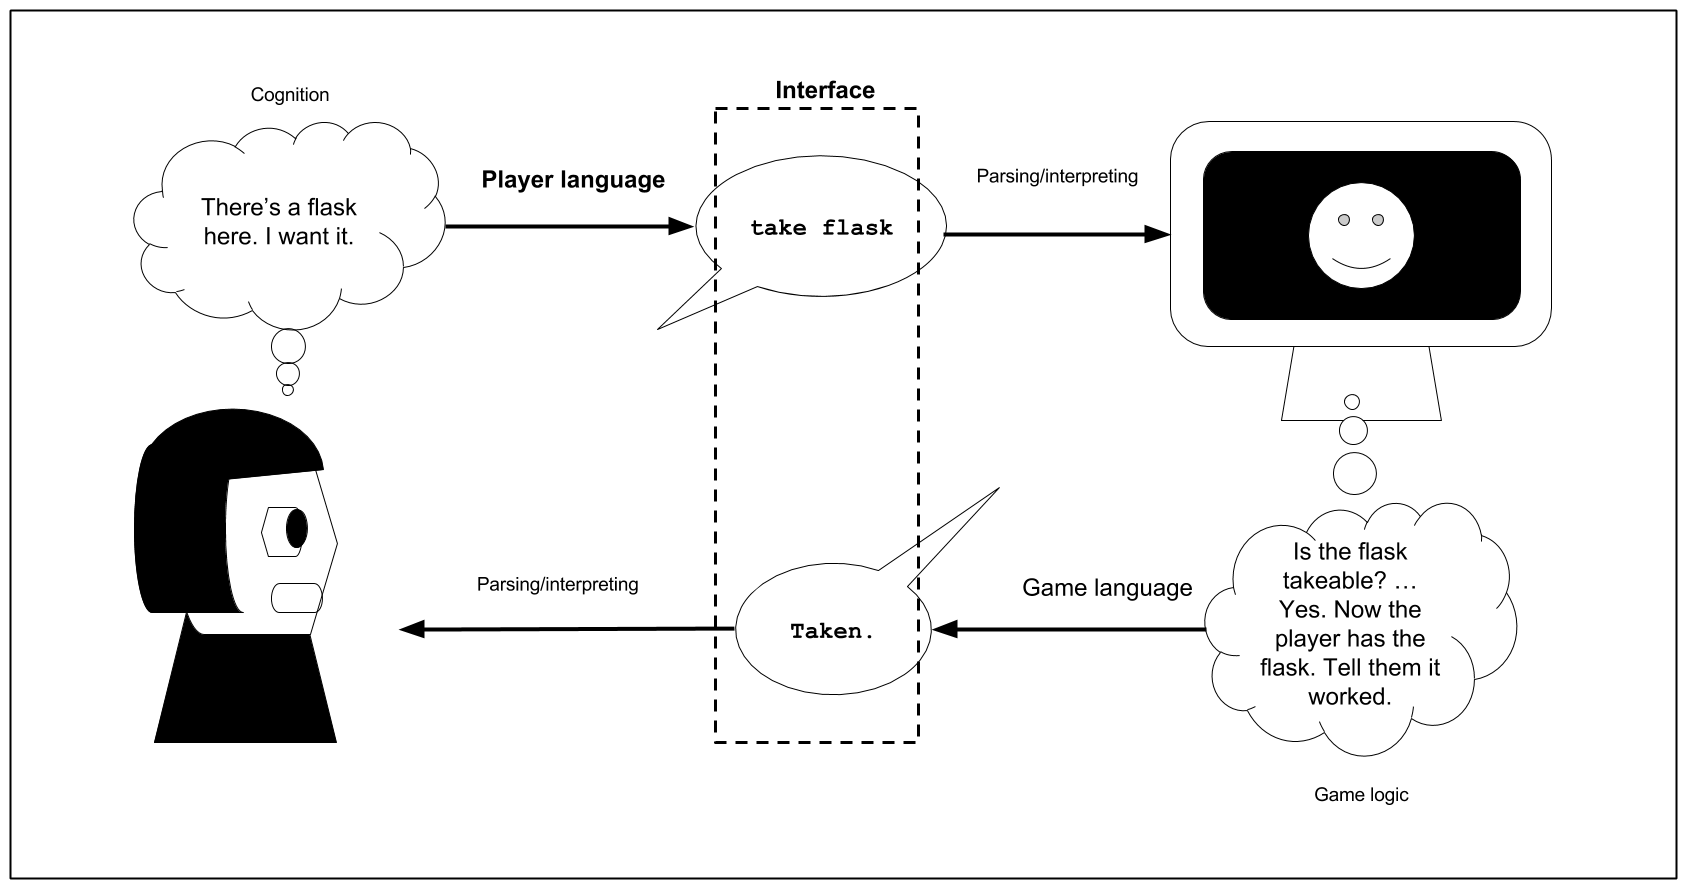
\includegraphics[width=0.75\textwidth]{conversation-processing.png}
\caption{A process diagram of a game loop: player and game conversation as
it relates to language, interface, and cognition.}
\label{fig:gameloop}
\end{figure*}

Since the constraints on what
language they may use are wholly determined by a piece of software (the
game interface), we argue that these languages more in common with a {\em
programming language} (PL) (broadly defined as a formal language whose meaning
is fully grounded in a computational system) than a natural language. 
Accordingly, each game in some sense {\em defines its own programming
language}. In a slogan, we could term this project {\em games as
programming languages}.

% What is to be gained by this analogy?

This analogy opens up a whole field of methodology to try applying to
games.  The programming languages (PL) community has a long and deep
history of assigning mathematically formal semantics to languages and
analyzing those semantics. As games researchers become more interested in
the emergent consequences of the systems they assemble, the tools of PL
theory have a lot to offer. For example, PL theory provides an account of
{\em compositionality}, i.e. how fragments of expression fit together to
form higher-level meanings. In games, this translates into being able to
understand player {\em skills} or strategies as compositions of player
actions, which we demonstrate in this paper by using a formalized input
language as a kind of ``player AI scripting language.''

% PL theory also
% provides an account of
% how to relate meaning in a {\em low level} representation (such as assembly
% language, or on the games side, control-level interactions) to meaning in a
% {\em high-level} language (such as a language like Java or a game's state
% space), allowing us to draw abstraction boundaries and consider system
% components in compositional terms. For example, we can consider what it
% means to have a game with the same {\em internal mechanics} (or what Salen
% and Zimmerman (XXX) call {\em constiutative rules}) but distinct interface,
% comparing the meaning of these interfaces on formal terms.


% In Salen and Zimmerman (XXX cite) terms,
% PL theory can help us formalize the {\em constituative mechanics} of a
% game's interface so that we may consider distinct {\em operational rules} 
% that interface with them. 

% XXX example: parser vs. hypertext interactive fiction?
%
% Parser:
%   Interface:
%     >
%   Recognized utterances - contextual:
%    > <verb> <noun>
%    > <verb>
%    > <verb> <noun> <preposition> <noun>
%
% Hypertext:
%   Interface: contextual, e.g.
%     [[go north]] or [[go south]] or [[take sword]] ?
%   Recognized utterances:
%     (link clicks) - 1 dimensional, contextual, ambiguous


Furthermore, by considering a player's language of expression as an object
of study in its own right, we center them as a co-designer of the experience
afforded by a game. When we treat a player's interactions as not simply an
arbitrary sequence of button presses that advances and reveals the
designer's intent, but instead as its own distinct {\em voice} that a game
system must listen and respond to, we enable the player to {\em co-create}
with the system, potentially developing deeper systems understanding
and emotional investment.

In the remainder of the paper, we concretize the analogy by introducing the
components of a theoretical account of a programming language (syntax, type
system, and operational semantics) and its analog in a game. We walk
through an example to illustrate how to think about a game in terms of its
language-like affordances, and we demonstrate the payoff of this line of
thought by extending the metaphor to account for {\em player skills} as
``programs,'' effectively representing mental models for how to accomplish
some task in terms of the game's linguistic constructs.

\section{Related Work}


Cardona-Rivera and Young~\cite{cardona2014games}
detailed a conceptual framework following the slogan {\em games as
conversation}, grounding the communicative strategies of games in cognitive
science for human-to-human conversational understanding, such as Grice's
maxims~\cite{grice1975logic}. They offer a linguistic and semiotic approach to
understanding how a game communicates affordances (possibilities for
action) to a player.  For an account of the game's half of the equation,
which includes the visual, textual, and audio feedback mechanisms intended
to be processed by the player, this application of linguistics, psychology,
and design seems appropriate, much like the study of cinematic language for
film.  On the other hand, we argue that a PL approach better supports
understanding of the player-to-game direction, since the language the
player speaks toward a digital game is formal and unambiguous.

Researchers have previously recognized the value in formalizing interaction
vocabularies, realizing certain interaction conventions as a {\em single}
``video game description language''~\cite{ebner2013towards} whose
implementation as VGDL~\cite{schaul2013video} has been used in game AI research. We
suggest instead that the design space of player languages is as varied as
the design space of programming languages and herein give an account of
what it would mean to treat each language individually.
Our project suggests that an appropriately expressive computational
framework analogous to VGDL should be one that can accommodate the encoding
of many such languages, such as a {\em meta-logical framework} like the
Twelf system for encoding and analyzing programming language
designs~\cite{pfenning1999system}. 

% AI action languages (planning, event calc, etc.); general game AI frameworks
Any investigation into formalizing actions within an interactive system
shares ideas with ``action languages'' in AI extending as far back as
McCarthy's situation calculus~\cite{mccarthy1969some} and including
planning languages and process calculi.  These systems have been studied in the
context of game design, e.g. the Ludocore system~\cite{smith2010ludocore};
however, AI researchers are mainly interested in these formalisms as internal
representations for intelligent systems and the extent to which they support
reasoning.  Conversely, we are interested their potential to support player
expression and facilitate human-computer conversation.

Some theoretical and experimental investigations have been carried out
about differences between game interfaces along specific axes, such as
whether the interface is ``integrated'' (or one might say diagetic), versus
extrinsic to the game world in the form of menus and
buttons~\cite{llanos2011players, jorgensen2013gameworld}. These
investigations suggest an interest in more detailed and formal ontologies
of game interfaces, which our work aims to provide.

(XXX transition)
Hazelnut is a formal model of a program editor that enforces that
every edit state is meaningful (it consists of a well-defined syntax
tree, with a well-defined type)~\cite{Omar17Hazelnut}.
%
Its type system and editing semantics permit \emph{partial programs},
which contain missing pieces and well-marked type inconsistencies.
%
Specifically, Hazelnut proposes a \emph{editing language}, which
defines how a cursor moves and edits the syntax tree; the planned
benefits of this model range from better editing assistance, the
potential to better automate systematic edits, and further
context-aware assistance and automation based on statistical analysis
of (semantically-rich) corpses of recorded past edits, which consist
of \emph{traces} from this language~\cite{Omar17Hazel}.
%
Likewise, in the context of game design, we propose a player language;
we expect similar benefits, as outlined elsewhere in the paper (??).

\paragraph{Functional reactive programming.}
%
Functional reactive programming (FRP) describes computations that
consume and produce time-varying data using techniques and ideas from
functional programming.
%
\citep{Fran,HudakEtAl,Cooper06embeddingdynamic,Krishnaswami11,Krishnaswami13,Czaplicki2013AFR}.




\section{A Framework}

  % Background: Syntax, type systems, and operational semantics
\newcommand{\param}[1]{\langle #1 \rangle}
\newcommand{\syn}[1]{\mathsf{#1}}


  In the formal study of a programming langugage, one may define a language
  in three parts: syntax, type system, and operational semantics.
  \begin{itemize}
    \item The {\em syntax} is written in the form of a (usually)
      context-free grammar describing the allowable expressions. One
      sometimes distinguishes between {\em concrete syntax}, the literal
      program tokens that the programmer strings together in the act of
      programming, and {\em abstract syntax}, the normalized ``syntax
      tree'' structures that ultimately get interpreted. 
    \item An {\em operational semantics} defines how runnable programs
      (e.g. a function applied to an argument) {\em reduce} to values. This
      part of the definition describes how actual computation takes place
      when programs in the language are run. It is important to note that
      the operational semantics need not reflect the actual {\em
      implementation} of the language, nor is it specific to a ``compiled''
      versus ``interpreted'' understanding of the language: it is simply a
      mathematical specification for how any compiler or interpreter for
      the language should behave.
    \item A {\em type system} further refines the set of syntactically
      valid expressions into a set of {\em meaningful} expressions, and provides
      a mapping between an expression and an approximation of its meaning.
      Type systems are usually designed in conjunction with the operational
      semantics to have the property that every expression assigned a
      meaning by the type system should have a well-defined runtime
      behavior. In practice, however, type systems can only approximate
      this correspondence. Some err on the more permissive side--e.g.
      C's type system will permit invalid memory accesses with no
      language-defined behavior--and some err on the more restrictive side,
      e.g. Haskell's type system does not permit any untracked
      side-effects, at the expense of easily authoring e.g. file input/output
      (without first learning the details of the type system).
  \end{itemize}
  
  Providing a formal language definition in programming languages research
  has several purposes. One is that it enables researchers to explore
  and prove formal properties of their language, such as {\em well-typed
  programs don't go wrong}, or in a language for concurrency, a property
  like deadlock freedom. However, an even more crucial advantage of a
  language specification is not mathematical rigor but human capacity to do
  science. A language definition is a {\em specification}, similar to an
  application programmer interface (API) or an IEEE standard: it describes
  an unambiguous interface to the language along an {\em abstraction
  boundary} that other human beings may access, understand, and implement,
  without knowing the internals of a language implementation.  It is a
  necessary component of reproducibility of research, and it allows
  researchers to build on each other's work. We believe that an embrace of
  the formal specification in games research can play a similarly important
  function.

  \begin{table}
  \begin{tabular}{l|ll}
    PL concept & Game concept\\
    \hline
    Syntax & Recognized player intents & (Section \ref{sec:syntax})\\
    Operational semantics & Game mechanics & (Section \ref{sec:opsem})\\
    Type system & Contextual interface & (Section \ref{sec:typesys})\\
    Straight-line programs & Play traces & (Section \ref{sec:traces})\\ 
    General programs & Player skills & (Section \ref{sec:skills})
    \\
    \hline
  \end{tabular}
%  \caption{Languages for player-game interfaces: Formal decomposition
 %   (left) and informal correspondances (right).}
  \caption{Player intent languages: 
    \\
    Formal decomposition (left) and correspondances (right).}
  \label{tab:correspondence}
  \end{table}

  Having provided loose definitions of these terms, we now wish to draw out
  the analogy between a {\em language} specification and a {\em game}
  specification. To treat a game in this manner, we wish to consider player
  affordances and actions, as well as their behavior (mechanics) in the
  context of the game's running environment. We summarize the components of
  this correspondence in Table~\ref{tab:correspondence}.

  \newcommand{\cmove}{\mathsf{move}}
  \newcommand{\ctake}{\mathsf{take}}
  \newcommand{\ccollect}{\mathsf{collect}}

  We will use as a running example a minimal virtual environment with two
  player actions: (1) movement through a discrete set of rooms in a
  pre-defined map ($\cmove$); (2) acquiring objects placed in those rooms to store in
  a player inventory ($\ctake$).  We consider five (somewhat aribitrary)
  possibilities in the design space of interfaces for such a game,
  summarized visually in Figure~\ref{fig:uis}:

  \begin{itemize}
   \item {\bf Point-and-Click:} A first-person viewpoint interface where the
     meaning of each click is defined based on the region the cursor falls
     in. Clicking near any of the four screen edges moves in that
     direction; clicking on a sprite representing an item takes it.
  \item {\bf Bird's-Eye:} A top-down viewpoint interface where the player can see multiple
    rooms at once, and can click on rooms and objects that are far away,
    but those clicks only do something to objects in the same room or
    adjacent rooms.
  \item {\bf WASD+:} A keyboard or controller-based interface with
    directional buttons (e.g. arrow keys or WASD) move an avatar in the
    correspondingi direction, and a separate key or button expresses
    the $\ctake$ action, which takes any object in the same room. (This
    interface may be used for either of the two views described above.)
  \item{\bf Command-Line:} The player interacts by typing free-form text, 
    which is then parsed into commands, such as \verb|take lamp| and \verb|move north|.
  \item{\bf Hypertext}: A choice-based interface where all available options are
    enumerated as textual links from which the player chooses.
  \end{itemize}

  \begin{figure*}
    \begin{tabular}{cc}
      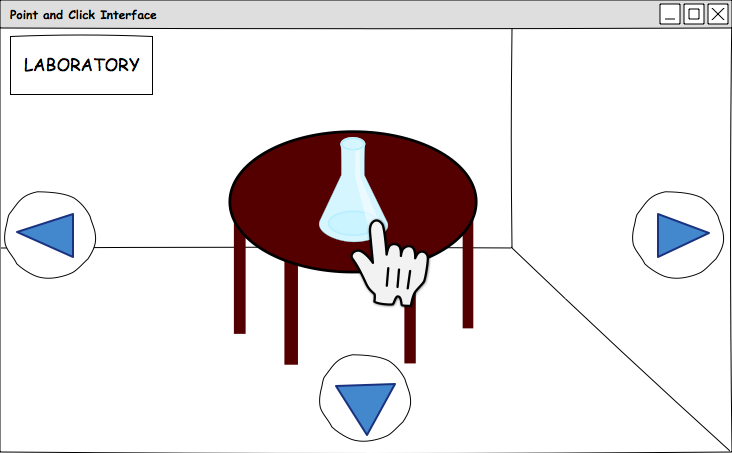
\includegraphics[height=0.2\textheight]{../uis/point-and-click.png} &
    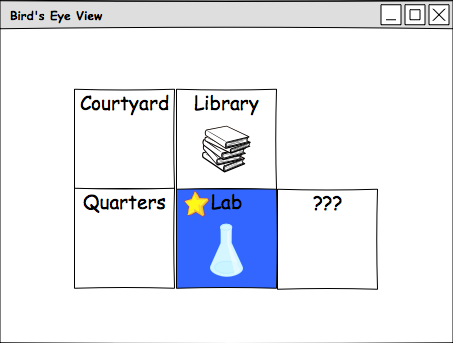
\includegraphics[height=0.2\textheight]{../uis/bev-color.png}
    \\
    Point-and-click & Bird's eye view/WASD+\\
    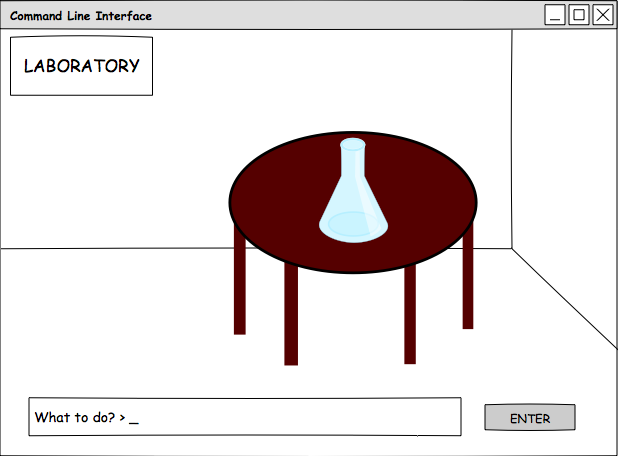
\includegraphics[height=0.2\textheight]{../uis/parser.png} &
    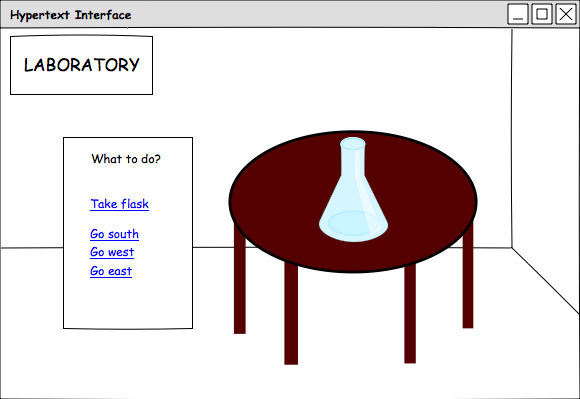
\includegraphics[height=0.2\textheight]{../uis/hypertext.png}\\
    Command-line & Hypertext
  \end{tabular}
  \caption{Four different user interfaces for the move/take game.}
  \label{fig:uis}
  \end{figure*}

  In the following sections, we will consider these possibilities in light
  of design choices relevant to the specified aspect of PL design.

  \section{Player intent as syntax}
  \label{sec:syntax}


%   \begin{figure*}
%     \begin{tabular}{|l|c|}
%       \hline
%       Language layer   & $\syn{move}(dir)$, etc. (XXX) \\
%       \hline
%       Affordance layer &
%         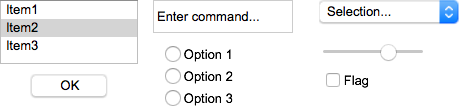
\includegraphics[width=0.5\textwidth]{ui-elements.png}\\
%       \hline
%       Device layer & 
%         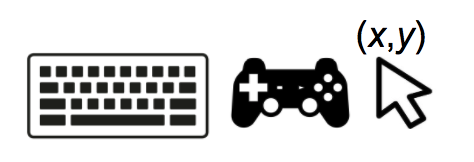
\includegraphics[width=0.4\textwidth]{control-devices.png}\\
%       \hline
%     \end{tabular}
%     \caption{XXX caption}
%     \label{fig:layers}
%   \end{figure*}
% 
% 
%   The {\em syntax} of a game is its space of recognized player commands.
%   However, this statement alone is imprecise: what counts as a {\em
%   command}, and what counts as {\em recognition}? Consider the
%   stratification of abstraction layers in Figure~\ref{fig:layers}: on the
%   hardware device level (which we consider out of scope for this paper),
%   the player issues a command by pressing, tapping, twisting, etc. 
%   physical buttons, keys, screens, and other tactile or embodied
%   affordances. This layer contends with the interactions between the
%   player's physical body and the game system. At the next layer up are
%   software affordances, or ``UI (user interface) elements:'' buttons,
%   sliders, menus, and other on-screen widgets that serve both to cue the
%   player ``interact with this'' and to {\em limit} the space of possible
%   hardware interactions (e.g. mouse clicks) to those that are relevant to
%   the particular software (e.g. buttons, check-boxes). Finally, the {\em
%   language} layer is closest to the game's mechanics themselves: the
%   recognized verbs, nouns, and other data relevant to a diagetic {\em
%   intent} that the player wishes to carry out.
% 
%   The two processing steps in this pipeline---device to affordance, and
%   affordance to language---resemble the distinction between concrete and
%   abstract syntax. An important difference between the two levels is
%   whether {\em context matters}: the keys on a keyboard may be pressed at
%   any time during a player's interaction with a computer; context within
%   the game world does not restrict their use. On the other hand, which menu
%   options are available may depend a great deal on context: if a player has
%   opened their inventory, different options may be available from those
%   available when looking at, say, an overworld map. Correspondingly,
%   context-independent actions are probably carried out
%   repeatedly---pressing arrow keys and space in a PC platformer using those
%   keys as controls, for example. On the other hand, their interpretation
%   one layer up---``jump onto the transport platform'' or ''fall down onto
%   (a specific) enemy NPC''---only make sense in very specific game world
%   contexts and are infrequently (or perhaps never) repeated.
% 
%   Where to draw the line between concrete and abstract is largely a matter
%   of choice that will determine how we can view and analyze a game.
%   In the following examples, we describe concrete syntax in terms of
%   anything a player can do that the game's audiovisual interface suggests
%   might be possible: e.g. if a mouse cursor is displayed whenever the
%   player moves the mouse, then we consider a mouse click anywhere on the
%   screen to be part of the concrete syntax. If a player is allowed to type
%   arbitrary text (or speak aloud arbitrary phonemes), and the game
%   interface displays or repeats back what the player said, then we consider
%   the concrete syntax to be those arbitrary sequences of characters or
%   phonemes.
% 
%   At the abstract layer, we 
%   

  The {\em syntax} of a game is its space of recognized player intentions.
  Note that {\em intention} is different from {\em action} in the sense
  that we don't necessarily expect each well-formed intention to change
  anything about the game state: a player can intend to move north, but if
  there is no room to the north of the player when she expresses this
  intent, no change to the game's internal state will occur. Nonetheless,
  depending on the design goals of the game, we may wish to recognize this
  as a valid intent so that the game may respond in some useful way (e.g.
  with feedback that the player cannot move in that direction).
  
  In our example game, the choice of syntax answers questions such as: can
  the player click anywhere, or only in regions that have meaning? Can the
  player type arbitrary commands, or should we provide a menu or
  auto-complete text so as to prevent the player from entering meaningless
  commands?  In PL, we can formalize these decisions by describing an {\em
  abstract syntax} for our language, which is typically assumed to be
  context-free and thus specified as a Bachus-Naur Form (BNF) grammar. Our
  examples below follow the interfaces shown visually in
  Figure~\ref{fig:uis}.
  
  \textbf{WASD+ Interface}:
  One way of writing the BNF for the WASD+ interface is:
  %
  \begin{eqnarray*}
  direction &::=& \mathsf{north} \mid \mathsf{south} \mid \mathsf{east}
    \mid \mathsf{west} \\
  intent &::=& \cmove \langle direction \rangle \mid \ccollect
  \end{eqnarray*}
  %
  The hardware interface maps onto this syntax quite directly:
  each arrow key maps onto a $\cmove$ action in the corresponding
  direction, and the specified other key maps onto $\ccollect$.

  \textbf{Bird's Eye View Mouse Interface}:
  On the other hand, a clicking-based interface to a top-down map could
  enable the player to click on any room on the map and any item within a
  room. This syntax would look like:
  %
  \begin{eqnarray*}
    room   &::=& \syn{courtyard} \mid \syn{library} \mid \syn{quarters}
              \mid \syn{lab}\\
    item   &::=& \syn{flask} \mid \syn{book}\\
    entity &::=& room \mid item\\
    intent &::=& \syn{click}\param{entity}
  \end{eqnarray*}
  %
  Note that this syntax, compared to that for WASD+, describes a larger set
  of possible utterances, even though it has the exact same set of
  permitted game behaviors (a player may only move into adjacent rooms and
  take items that share a room with them). 

% XXX make this point at the end of the section
%   The {\em size} of the player
%   intent language, i.e. the number of distinct intents it is possible to
%   form and express through the game language, constitutes a significant
%   aspect of the game design. A game with fewer expressible intents might
%   feel easier, and conversely less exploratory: the player is only allowed
%   to speak utterances that the game is guaranteed to validate. 

  \textbf{Command Line Interface}:
  The command-line interface would have an even larger space of expressible
  utterances if we consider all typed strings of characters to be valid
  expressions, but that syntax is too low-level for linguistic
  considerations. Supposing we interpose a parsing layer between arbitrary
  typed strings and syntactically-well-formed commands, we can define the
  abstract syntax as follows (where $direction$ and $item$ are assumed to
  be defined as they were in the previous examples):
%
  \begin{eqnarray*}
    intent &::=& \cmove\param{direction} \mid \ctake\param{item}
  \end{eqnarray*}
%
  Assuming the player ``knows the language,'' i.e. knows that $\cmove$
  and $\ctake$ are valid commands, and in fact the {\em only} valid
  commands, and assuming that she knows how to map the visual affordances
  (e.g. image of the flask) to the typed noun (e.g. \verb|flask|), the
  experience afforded by this interface is quite similar to the WASD+
  interface. The main difference is that the player must specify an {\em
  argument} to the $\syn{take}$ command, asking the player to formulate a
  more complete (and unambiguous) intent by actually naming the object she
  wishes to take.

%   When a player sees an empty command prompt as an interface to a game, she
%   may try using another language she knows, such as one used in classic
%   interactive fiction that recognizes a wide space of valid imperative
%   sentences:
%   \begin{eqnarray*}
%     intent &::=& iverb \mid
%                  tverb\param{noun} \mid
%                  \syn{go}\param{direction} \\
%              &\mid& \syn{put}\param{noun}\syn{\ on}\param{noun} \\
%              &\mid& \syn{strike}\param{noun}\syn{\ with}\param{noun}\\
%              &\mid& \hdots\\
%     iverb &::=& \syn{look} \mid \syn{listen} \mid \syn{wait} \mid \hdots\\
%     tverb &::=& \syn{take} \mid \syn{examine} \mid \syn{drop}\mid \hdots
%   \end{eqnarray*}



  \textbf{Hypertext interface}:
  Finally, we consider the intent language for the hypertext interface.
  This is one of the most difficult interfaces to formulate in linguistic
  terms, because it either requires that we formalize link selection in an
  acontextual way (e.g. as a numeric index into a list of options of
  unknown size) or that we formulate each link {\em from each page} as its
  own separate command, each of which has meaning in only one specific game
  context (namely, when the player is on the page containing that link).
  The former feels like a more general formulation of hypertext that is not
  relevant to any particular game, and since we are aiming to provide a
  correspondence between specific games and languages, we opt for the
  latter:
  %
  \begin{eqnarray*}
    intent &::=& \syn{select}\param{choice}\\
    choice &::=& \syn{take\_flask\_from\_lab}\\
           &\mid& \syn{take\_book\_from\_library}\\
           &\mid& \syn{go\_south\_from\_lab} \\
           &\mid& \syn{go\_east\_from\_lab} \\
           &\mid& \syn{go\_west\_from\_lab} \\
           &\mid& \syn{go\_north\_from\_library} \\
           &\mid& \hdots
  \end{eqnarray*}
  %
  Some hypertext authors put a lot of effort into scaffolding the
  choice-based experience with a richer language, e.g. by repeating the
  same set of commands across different pages that behave in consistent
  ways, or by creating menu-like interfaces where text cycles between
  options on an otherwise static page. In this way, hypertext as a medium
  might be said as providing a playform for designers to create their own
  interface conventions, rather than relying on a set of pre-established
  ones; by the same token, hypertext games created by inexperienced
  interface (or language) designers may feel to players like being asked to
  speak a foreign language for each new game.

  \subsection*{Additive and subtractive properties of syntax}
  
  By now we are able to observe that, just like the rest of a game's rules,
  its syntax has both additive and subtractive properties. It provides the
  menu of options for which hardware interactions are {\em relevant}, i.e.
  likely to result in meaningful interaction with the game system, but it
  also establishes which utterances within that set are {\em disallowed},
  or ill-formed---e.g. that it is not meaningful to say ``take'' without
  providing an object to the command, or that ``take north'' is ill-formed.

  Correspondingly, an important decision that impacts game design is (a)
  how discoverable the additive affordances are (e.g. can the player
  determine that ``examine'' is a meaningful verb without already
  possessing literacy in the game's genre?) and (b) the extent to which the
  user interface makes meaningless expressions impossible to form. For
  example, in a hypertext interface, all links lead somewhere---so every
  intent the player can form, i.e. clicking a link on the page, will get a
  valid response from the game, whereas ``take fnord'' typed at a
  command-line interface may be recognized by the parser, but meaningless
  to a game where ``fnord'' is not a noun.  Decisions about these two
  (related) dimensions will determine the extent to which {\em learning the
  language}, an exploratory but sometimes frustrating process, is a central
  challenge of the game.
  


  \section{Game mechanics as \\ operational semantics}
  \label{sec:opsem}

%  (XXX move this before or after opsem part?)
%  \subsection{Game environment as external runtime}

%  To characterize mechanics, we will also need an account of expressions
%  permissible in the game's language (e.g. display a room, make a sound,
%  make an object disappear, etc. --- things more commonly accounted for in
%  formal game description languages). 

%  (XXX more; transition?)
%   We will also need to characterize ``hidden'' state of the game...
%   predicate syntax... locations of things, adjacency graph to describe the
%   world map
% 
%   World state $\sigma$; game expressions $e_g$; used in the judgments
%   defining operational semantics below

  \newcommand{\Player}[4]{\ensuremath{#1{:}\left< {#2} , {#3} , {#4} \right>}}
\newcommand{\PropIsTrue}[2]{\ensuremath{#1 \vdash #2~\textsf{true}}}
\newcommand{\StepsTo}[4]{\ensuremath{\left< #1 ; #2 \right> \longrightarrow \left< #3 ; #4 \right>}}

\section{Precise player-game dynamics via operational semantics}
\label{sec:opsem}

The player consists of a 

The operational semantics employs notions of the game and player states.

The following BNF definitions give meta variable conventions (the left-hand-side variable names) and syntactic cases (the right-hand-side of each rule).


\begin{figure*}
\small

\begin{tabular}{l|l}

\begin{minipage}{0.7\textwidth}
\begin{tabular}{lccll}
propositions   & $P$ & $::=$ & $\cdots$ & Game world propositions~(See~$\PropIsTrue{G}{P}$)
\\
player command & $C$ & $::=$ & $\cdot$ $~|~$ $c$ & Unit and atomic commands (0 and 1 turns, resp.)
\\
               &     & $~|~$ & $C_1~{;}~C_2$ & Command sequences (multi-turn commands)
\\
               &     & $~|~$ & $\textsf{until}~P~\textsf{do}~C$ & Command loops (e.g., for player skills)
\\
atomic command & $c$ & $::=$ & $\textsf{grasp}~i$ & Attempt to place~object$i$ into player's hand
\\
               &     & $|$   & $\textsf{drop}$ & Drop the held object, if any
\\
               &     & $|$   & $\textsf{giveTo}~i$ & Give held object to another~(named~$i$)
\\
               &     & $|$   & $\textsf{takeFrom}~i$ & Take hold of object from another~(named~$i$)
\\
               &     & $|$   & $\textsf{moveTo}~i$ & Move adjacent to object, place or agent~(named~$i$)
\\
               &     & $|$   & $\textsf{moveThrough}~i$ & Move through opening~(named~$i$)
\\[5mm]
unique IDs & $i,j$ & $::=$ & $\cdots$ & (\emph{abstract}, e.g., numbers, symbols, noun phrases)
\\
game state & $G$ & $::=$ & $\cdots$ & (\emph{abstract})
\\
player state & $p$ & $::=$ & $$ & Player identity, bag~$B$, hand~$h$ and commands~$C$
\\
unit space (hand) & $s,h$ & $::=$ & $\square~|~i$ & An empty space, or an object~(named~$i$)
\\
aggregate space (bag) & $S,B$ & $::=$ & $\cdot~|~s::S$ & Zero or more unit spaces
\end{tabular}
\end{minipage}

&

\begin{minipage}{0.3\textwidth}
\[
\begin{array}{ll}
\fbox{$G_1 \equiv G_2$}~\textrm{World equivalence}
\\
\fbox{$b_1 \equiv b_2$}~\textrm{Bag equivalence}
\\
\fbox{$\PropIsTrue{G}{P}$} 
\\
\textrm{In world~$G$, proposition~$P$ is true}.
\\[2mm]
\fbox{$\StepsTo{G}{p}{G'}{p'}$}
\\[2mm]

\infer
{  
\StepsTo
{G}{\Player{i}{B_1}{\square} {\textsf{grasp}~$j$}}
{G}{\Player{i}{B_2}{j}{\cdot}}
}
{
B_1 \equiv j :: B_2
}


\end{array}
\]
\end{minipage}


\end{tabular}

\caption{Definitions for an operational semantics: Captures precise
  player-game dynamics for a primitive adventure game.}
\end{figure*}


  \section{Contextual interfaces as \\ type systems}
  \label{sec:typesys}

  Decisions about interface syntax can, to some extent, limit or expand the
  player's ability to form intents that will be met with failure, such as
  moving through a wall or taking an object that does not exist. But
  sometimes, whether an utterance is {\em meaningful} or not will depend on
  the runtime game state, and can be considered a distinct question from whether it is
  well-formed. For example, whether or not we can {\em take
  flask} depends on whether the flask is present, but if the flask is an
  object somewhere in the game, we must treat this command as well-formed {\em
  syntax} and relegate its failure to integrate with the runtime game
  environment to the {\em mechanics} (operational semantics).

  However, some user interfaces nonetheless restrict the set of recognized
  utterances in a way that depends on current game state. Consider a
  point-and-click interface that changes the shape of the cursor to a hand
  whenever it hovers over an interactable object, and only recognizes
  clicks when it is in this state. Alternatively, consider the hypertext
  interface, which only recognizes clicks on links made available in the
  current page.  Providing the player with {\em only the option of saying}
  those utterances that ``make sense'' in this regard corresponds to a
  strong static type system for a programming language.

  Type systems are typically formalized be defining a relation between
  expressions $e$ and contexts $\Gamma$. Contexts are sets of specific
  circumstances in which an expression is valid, or well-typed. Usually,
  these circumstances have to do with {\em variables} in the program. For
  example, the program expression $x+3$ is only well-typed if $x$ is
  a number. ``$x$ is a number'' is an example of a fact that would be
  contained in the context. Its well-typedness could be represented as
  $x{:}\mathsf{num} \vdash x+3{\ \mathsf{ok}}$.
  
  In the move-take game, we can include aspects of game state in our
  context, such as the location of the player and the adjacency mapping
  between rooms in the world. An example of a typing rule we might include
  to codify the ``only present things are takeable'' rule would be:
  % No whitespace here
  \[
    \infer
    { 
      \Gamma \vdash \ctake\param{O}\ \syn{ok}
    }
    {
      \Gamma \vdash \syn{playerIn}(R)
      \quad
      \Gamma \vdash \syn{at}(O, R)
    }
  \]
  %
  We then need to define a relation between concrete game states $G$ and
  abstract conditions on those states, $\Gamma$. We might write this
  relation $G\ :\ \Gamma$.
  After such rules are codified, we can refine the ``game completeness''
  conjecture to handle only those utterances that are well-typed:
  %
  \[
  \begin{array}{cc}
  \forall G_1, \mathit{intent}.
  & (G_1\ :\ \Gamma)
    \land
    (\Gamma \vdash intent\ \syn{ok})
  \\
\Longrightarrow
  \exists G_2, \mathit{resp}.
  &\GameStep
    {G_1}{\mathit{intent}}
    {G_2}{\mathit{resp}}
  \end{array}
  \]
  %
  This is nearly what we want to know about our game mechanics.
  %  
  However, we want to apply this reasoning iteratively as the game progresses, so that we
  reason next about the player intention that leads from game state~$G_2$
  to another possibly different game state~$G_3$; but what context for player intent describes state~$G_2$?
  
  For this reasoning to work, we generally need to update the original context~$\Gamma$,
  possibly changing its assumptions, and creating~$\Gamma'$.  We write $\Gamma \subseteq \Gamma'$ to mean that $\Gamma'$ \emph{succeeds} $\Gamma$ in a well-defined way. 
  %
  We now want to show that, given a game state~$G_1$ and player intention~\ensuremath{\mathit{intent}} that agree about the context of assumptions~$\Gamma$, there exists a successor context~$\Gamma'$ that agrees with the new game state~$G_2$:
  %
  \[
  \begin{array}{lll}
  \forall G_1, \mathit{intent}.
  & (G_1\ :\ \Gamma)
    \land
    (\Gamma \vdash intent\ \syn{ok})
\\[2mm]
\Longrightarrow
 \exists \Gamma', G_2, \mathit{resp}.
  &
  \big( \GameStep
    {G_1}{\mathit{intent}}
    {G_2}{\mathit{resp}}
  \big)
\\
&
\wedge 
  (G_2  :\ \Gamma') 
\wedge 
  (\Gamma \subseteq \Gamma') 
\\
  & 
  \end{array}
  \]

  \section{Play traces as \\ straight-line programs}
  \label{sec:traces}

  
%  Argument for having a syntactically-well-founded structured term for a
%  play trace (XXX)

    If we consider the analogy of game interfaces as programming languages,
    the natural question arises, what is a {\em program} written in this
    programming language? We want to at least consider individual, atomic
    player actions to be complete programs; the preceding text provides
    such an account. But typical programs are more than one line
    long---what does it mean to sequence multiple actions in a game
    language?

    In a typical account of an imperative programming language, we
    introduce a sequencing operator $;$ where, if $c_1$ and $c_2$ are
    commands in the language, then $c_1;c_2$ is also an command.
    The operational semantics of such an command involves the
    composition of transformations on states $\sigma$:
    %
    \[
      \infer{
        \left< \sigma; (c_1;c_2)\right> \longrightarrow
        \sigma_2
      }
      {
        \left<\sigma; c_1 \right> \longrightarrow
          \sigma_1
        \quad
        \left<\sigma_1; c_2 \right> \longrightarrow
          \sigma_2
      }
    \]
    %
    However, interactive software makes this account more complicated by
    introducing the program response as a component. Instead of issuing
    arbitrary commands in sequence, the player may wait for a response or
    process responses in parallel with their decisions. In this respect, a
    player's ``programming'' activity more closely resembles something like
    live-coding than traditional program authoring. Execution of code
    happens alongside its authorship, interleaving the two activities. If
    we consider a round-trip through the game loop after each individual
    command issued, then what we arrive at is a notion of program that
    resembles a {\em play trace}: a log of player actions and game
    responses during a play session, e.g.
    \begin{quote}
      PLAYER: go north\\
      GAME: failure\\
      PLAYER: take flask\\
      GAME: success\\
      PLAYER: go south\\
      GAME: success
    \end{quote}
    Depending on the richness of our internal mechanics model, this play
    trace may contain useful information about changes in internal state
    related to the preconditions and effects of player actions. But the
    main important thing to note is that, despite the informal syntax used
    to present them here, these traces do not consist of strings of text
    entered directly by the player or added as log information by the game
    programmer---they are structured terms with abstract syntax that may be
    treated to the same formal techniques of interpretation and analysis as
    any program. And this syntax is at a high level of game-relevant
    interactions, not at the level of hardware inputs and engine code.

    Researchers in academia and the games industry alike have in recent
    years been increasingly interested in play trace data for the sake of
    analytics, such as understanding how their players are interacting with
    different components of the game and responding to this game with
    updates that support player interest~\cite{el2013game}. 
    For the most part, this trace data is collected through telemetry or
    other indirect means, like game variable monitoring, after which it
    must be analyzed for meaning.~\cite{Canossa2013} More recently,
    systems of structured trace terms that may be
    analyzed with logical queries have been
    proposed,~\cite{osborn2015playspecs} identifying as a benefit an
    ability to support automated testing at the level of design intents.
    Our PL analogy supports this line of inquiry and warrants
    further comparison and collaboration.

%   \section{Theorems?}
% 
%   While it is not often considered of high priority for game designers to
%   prove theorems about their software, and in fact a rich culture is
%   enjoyed around the concept of {\em glitches} in games programs, a
%   meticulous designer may still wish to understand the scope, complexity,
%   and compatibility of her game approximated by compatibility between 
%   player affordances and game rules. A formal examination of the game's
%   properties, when studied as a programming language, can provide just
%   that:
% 
%   Well-typed programs don't go wrong ~= every possible player utterance has
%   a defined meaning within the game rules
% 
%   XXX example of this failing?





  
% \section{Example}
% To test the extent to which this analogy holds beyond a smallest example,
we attempt to describe the logic of a complex resource economy game with
an extensive player language. In {\em Stardew Valley} (XXX cite), the
player has an inventory that permits varied interactions with the world,
beginning a number of tools for farming (axe, hoe, scythe,
pickaxe) which do different things in contact with the resources in the
surrounding environment; most include extracting some resource (wood,
stone, fiber, and so on), which themselves enter the player's inventory and
can be used in further interaction with the game world. There are also
context-sensitive interactions between the player and non-player characters
(NPCs), interfaces through which new items may be purchased (shops), and
mini-games including fishing.

While a full account of the language that this game affords the player is
beyond the scope of this paper, what follows is an attempt to include a
representative sample of the actions and affordances found in this game,
presented in terms of the framework described above.

(XXX summarize what we are doing in this section)

\subsection{Syntax}

% move, apply tool, interact (open chests, talk to people, open doors,
% sleep)
% eating, giving things to npcs

(XXX concrete vs. abstract syntax analog to controls vs. player actions?)

\newcommand{\param}[1]{\langle #1 \rangle}
\newcommand{\syn}[1]{\mathsf{#1}}

(an item is something held, an entity is something in the world)
\begin{eqnarray*}
action &::=& \syn{select} \param{item}\\
       &\mid& \syn{apply} \param{entity}\\
       &\mid& \syn{inquire} \param{entity}\\
       &\mid& \syn{move\_near} \param{entity}\\
       &\mid& \syn{move\_offscreen} \param{direction}
\end{eqnarray*}

While it would be tempting to use the syntax layer to encode the kind of
higher-level actions performed in the game most frequently---tilling land,
planting seeds, conversing with NPCs---we want to accurately reflect the
{\em extensibility} of Stardew Valley's player language by describing the
general system from which these actions are derived. In other words, rather
than having each instance of such an action be a special case that a player
must learn how to speak as an independent vocabulary term, instead, they
learn it through {\em composing} the pre-existing constructs of selecting items
and applying them to objects in the world. For example: (XXX explain this
more)

Higher-level actions:
\begin{verbatim}
action hoe = select hoe; move_near shrub; apply shrub
action mine = select pickaxe; move_near rock; apply rock
action enter_shop = move_near shop; inquire door(shop)
action talk = move_near npc; inquire npc
action plant = select seeds; move_near tilled_ground; apply tilled_ground
\end{verbatim}

\subsection{Context Dependence}

include discussion of whether the above sequences of actions will actually
succeed or not; protocols...

include discussion of inventory menu, shops, crafting, recipes, other contextual menus
(XXX here or later?)

\subsection{Semantics}

(We can probably just describe these in prose rather than writing out the
syntax in full)

XXX define predicates like extracts, cost of crop, etc?

% apply tool depends on the tool and the thing you apply it to;
% mining yields stone, copper
% chopping tree yields wood (nondeterministic: seeds, sap, acorns, etc.)
Case $\syn{apply}\param{entity}$:\\
If the player is near an object that can be {\em extracted} with the
applied tool (e.g. a tree may be extracted by an axe; stone and ores may be
extracted by the pickaxe), compute and display a state change removing that object and
replacing it with its drops. \\
If the player is not near such an object, compute and display nothing.

XXX say something about drops being random

The game has some internal rules that will detect collisions between the
player and dropped items to add them to her inventory (these collision
rules are not part of the player language, since they occur passively).

Case $\syn{move}\param{direction}$:\\
Change the player location (XXX mention above caveat re collisions)


Case $\syn{inquire}\param{object}$:\\
XXX

crops yield money

money can buy things in stores

recipe menu

interact depends on whether a person, chest, door, other game object




\section{Player skills as programs}
\label{sec:skills}

While considering ``straight-line'' traces may have some utility in player
analytics, a more exciting prospect for formalizing game interactions as
program constructs is the possibility of
encoding {\em parameterized} sequences of actions that may carry out
complex tasks. After all, games with rich player action languages afford
modes of exploratory and creative play: consider item crafting in
Minecraft~\cite{minecraft}, puzzle solving in Zork~\cite{blank1980zork}, or
creating sustainable autonomous systems like a supply chain in
Factorio~\cite{factorio}, a farm in Stardew Valley~\cite{stardew}, or a
transit system in Mini Metro~\cite{minimetro}.  Each of these activities
asks the player to understand a complex system and construct multi-step
sequences of actions to accomplish specific tasks. From the player's
perspective, these plans are constructed from higher-level activities,
such as {\em growing a crop} or {\em constructing a new tool}, which
themselves are constructed from the lower level game intent language.

A language, as we have formalized it, gives us the atomic pieces from which
we can construct these sequences, like Lego bricks can be used to construct
reconfigurable components of a house or spaceship. {\em Compositionality}
in language design is the principle that we may understand the meaning and
behavior of compound structures (e.g. sequences) in terms of the meaning
and behavior of each of its pieces (e.g. actions), together with the
meaning of how they are combined (e.g. carried out one after the other, or
in parallel). In this section, we describe how we might make sense of {\em
player skills} in terms of programs written in a more complex version of
the player language.

\begin{figure}
  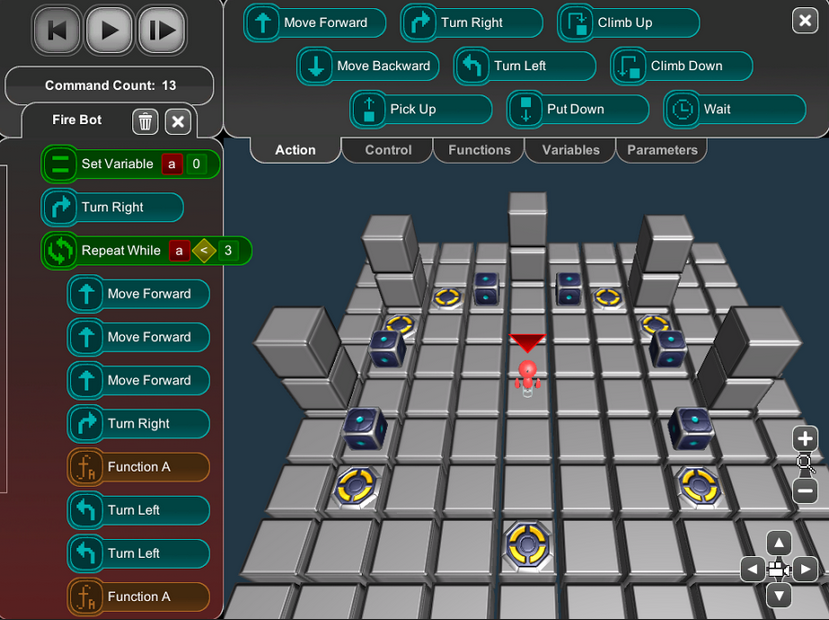
\includegraphics[width=0.45\textwidth]{bots.png}
  \caption{A screenshot from BOTS, an educational game in which players
  write programs to direct a player avatar.}
  \label{fig:bots}
\end{figure}

Such programs might be integrated into a game's mechanics so that a player
explicitly writes such programs, as in the BOTS game, an interactive
programming tutor that asks players to write small imperative programs that
direct an avatar within a virtual world~\cite{hicks2012creation} (see
Figure~\ref{fig:bots}), or Cube
Composer\footnote{\url{http://david-peter.de/cube-composer/}}, in which
players write functional programs to solve puzzles. However, for now, we
primarily intend this account of player skills as a conceptual tool.

\subsection{Example: Stardew Valley}

\begin{figure}
  
\includegraphics[width=0.45\textwidth]{stardew-valley.png}
  \caption{A screenshot from Stardew Valley showing the player's farm,
  inventory, and avatar.}
  \label{fig:stardew}
\end{figure}

Our initial $\{\cmove, \ctake\}$ example is too simple to craft really
compelling examples of complex programs, so here we examine
Stardew Valley and its game language for the sake of considering player
skills. In Stardew Valley, the player has an inventory that permits varied
interactions with the world, beginning with a number of tools for farming (axe,
hoe, scythe, pickaxe) which do different things in contact with the
resources in the surrounding environment; most include extracting some
resource (wood, stone, fiber, and so on), which themselves enter the
player's inventory and can be used in further interaction with the game
world. The player's avatar is shown on-screen, moved by WASD.  There are
also context-sensitive interactions between the player and non-player
characters (NPCs), interfaces through which new items may be purchased
(shops), and mini-games including fishing (fish may also be sold at high
value). See Figure~\ref{fig:stardew} for a typical player view of the game.

While a full account of the language that this game affords the player is
beyond the scope of this paper, we include a representative sample of the
actions and affordances found in this game that may be used to construct
player skills.
These include: directional avatar movement within and between
world ``rooms,'' point-and-click actions for selecting items in
one's inventory, and interacting with in-room entities. 

The player avatar must be near an entity for the player to interact with
it. They can then either $\syn{apply}$ the currently-selected inventory
item to the in-world entity with a left-button click, or right-button
click, which does something based on the entity type, e.g. doors and chests
open, characters speak, and collectible items transfer to the player's
inventory. We refer to this last action as $\syn{inquire}$. We also note
that, for the sake of our example, movement towards an entity and movement
offscreen (towards another room) are the only meaningful and distinct types
of movement, which we refer to as $\syn{move\_near}$ and
$\syn{move\_offscreen}$. These actions yield the following syntax:
%
% (an item is something held, an entity is something in the world)
\begin{eqnarray*}
intent &::=& \syn{select} \param{item}\\
       &\mid& \syn{apply} \param{entity}\\
       &\mid& \syn{inquire} \param{entity}\\
       &\mid& \syn{move\_near} \param{entity}\\
       &\mid& \syn{move\_offscreen} \param{direction}
\end{eqnarray*}
%
We leave the definition of items and entities abstract, but we could
imagine it to simply list all possible items and entities in the world as
terminal symbols.  
%
From these atomic inputs, we can start to construct higher-level actions
performed in the game most frequently---tilling land, planting seeds,
conversing with NPCs, and so on. These blocks of code may be assigned names
like functions to be called in many contexts:
%
% we want to accurately reflect the
% {\em extensibility} of Stardew Valley's player language by describing the
% general system from which these actions are derived. In other words, rather
% than having each instance of such an action be a special case that a player
% must learn how to speak as an independent vocabulary term, instead, they
% learn it through {\em composing} the pre-existing constructs of selecting items
% and applying them to objects in the world. For example: (XXX explain this
% more)
% 
% XXX semantics?
%
% Higher-level actions:
\begin{verbatim}
action till  = select hoe; move_near hard_ground; 
               apply hard_ground
action plant = select seeds; move_near tilled_ground; 
               apply tilled_ground
action mine  = select pickaxe; move_near rock; apply rock
action talk  = move_near npc; inquire npc
action enter_shop = move_near shop; inquire door(shop)
\end{verbatim}
%
In turn, these larger skill molecules may be combined to accomplish
specific tasks or complete quests.

\subsection{Branching programs as skills and strategies}

Note that we have naively sequenced actions without consideration for the
game's response. This approach to describing player skills does not take
into account the possbility of a failed attempt, such as attempting to mine
when there are no rocks on the current screen. One could simply assign a
semantics to these sequences of action that threads failure through the
program---if we fail on any action, the whole compound action fails.

However, we can go further with describing robust player skills and
strategies if we consider the possibility of {\em handling} failure, a
common feature of day-to-day programming and indeed of gameplay. Recall our
simplified game response language consisting of two possibilities,
$\syn{success}$ and $\syn{failure}$. We can introduce a $\syn{case}$
construct into our language to handle each of these possibilities as a
distinct branch of the program:
%
\begin{verbatim}
action mine = 
  response = select pickaxe;
  case(response):
    success => {
      response' = move_near rock;
      case(response'):
          success => apply rock;
        | failure => fail;
    }
  | failure => fail;
\end{verbatim}
%
However, to avoid handling failure at every possible action, a better
approach is to explicitly indicate as parameters the world resources that
each action needs in order to complete successfully.
The overall action definition for mining, or example, would
require as a precondition to the action that a pickaxe is
available in the player inventory and a rock is in the same room. The
actions for selecting the pickaxe and moving near the rock would depend on
these resources, and the game response language could include the resources
it guarantees as outputs. Then we can write the program using simpler
notation that refers to resource dependencies of the appropriate type
(using notation \verb|resource : type|):
%
\begin{verbatim}
action mine(p:pickaxe, r:rock) = 
  select p; move_near r; apply r
: mineral
\end{verbatim}
%
% The task of defining a language of compound actions enters novel territory
% in programming language design, because compound player actions
% are typically interleaved with game response: the player does not have full
% knowledge of how the game world works, so she experiments with its
% affordances, develops a model for which actions map to which responses, and
% then plans accordingly. 
% Players therefore often create ad-hoc plans on the basis of
% real-time game responses, gradually learning to form complex plans by
% thinking further in advance about their consequences.

This notation together with a branching \verb|case| construct
scales to include nondeterminism in the game world, such as the fishing
minigame in Stardew Valley: the game always eventually tells the player
that something is tugging at her line, but some portion of the time it is a
fish while the rest of the time it is trash.  These constructs can also
account for incomplete player mental models, such as knowing that one must
water her seeds repeatedly day after day in order to grow a crop, but not
knowing how many times.

Below, we present a notation that accounts for these aspects of player
skills: a \verb|do ... recv ...| notation indicates a command and then
binds the response to a {\em pattern}, or structured set of variables,
which can then be case-analyzed.
Our first example is watering a crop until it may be harvested:
%
\begin{figure}[t]
  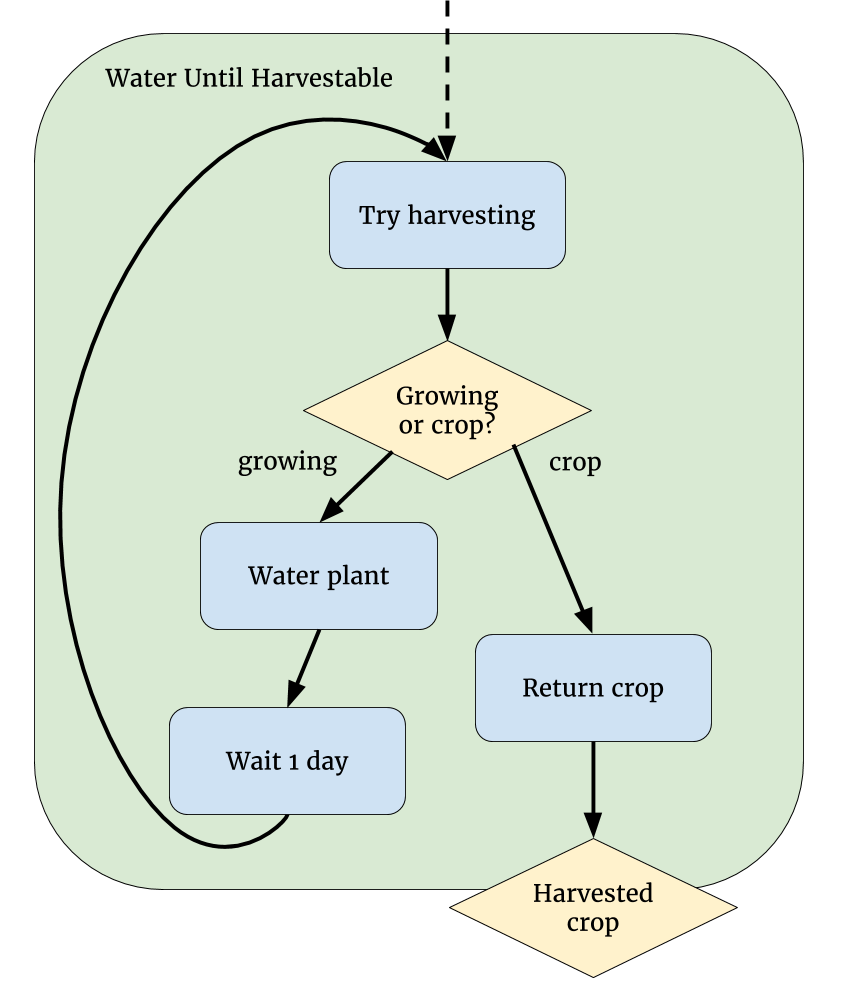
\includegraphics[width=0.4\textwidth]{sdv-water-harvest.png}
  \caption{Watering a crop until it may be harvested.}
  \label{fig:harvest}
\end{figure}
%
\begin{verbatim}
action water_until_harvestable[t](p: planted(t))
: crop(t) =
  do try_harvest(p)
    recv <result: crop(t) + growing(t)>.
      case result of
        c:crop(t) => c
      | g:growing(t) => 
          water(g); 
          wait(day); 
          try_harvest(g)
\end{verbatim}
See Figure~\ref{fig:harvest} for a control flow diagram of this code.

The next example shows a parallel construct \verb/||/, which can be used to
compose actions with distinct dependencies, as well as
how an action definition may use other action definitions by threading
resource dependencies through as arguments:
%
\begin{figure}[t]
  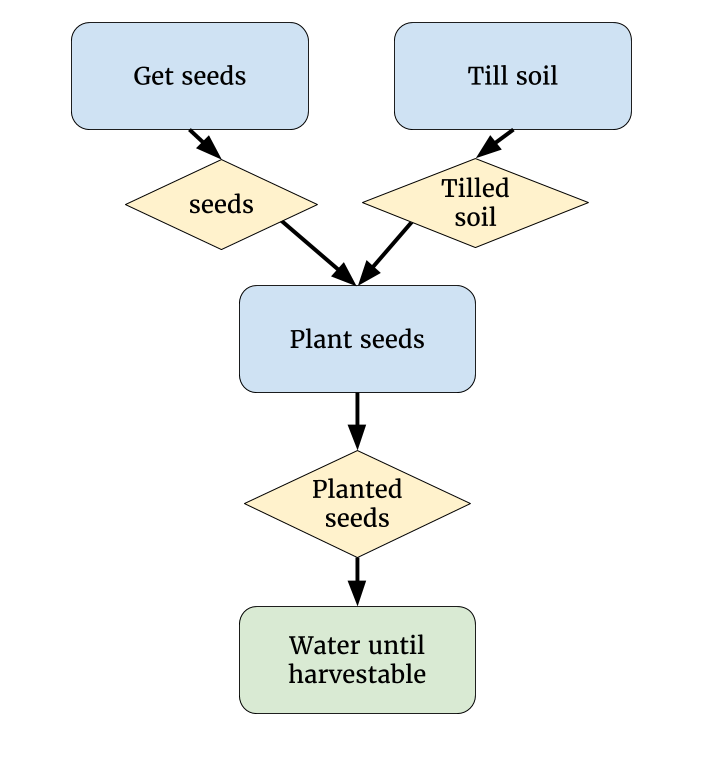
\includegraphics[width=0.4\textwidth]{sdv-grow-crop.png}
  \caption{Growing a crop.}
  \label{fig:grow}
\end{figure}
%
\begin{verbatim}
fun grow_crop[t : croptype](s:soil, w:watering_can)
: crop(t) =
  do
    get_seeds(t) || till_soil(s)
  recv <s: seeds(t), g: tilled_soil>.
    do
      plant(s, g)
    recv <p: planted(t)>.water_until_harvestable(p)
\end{verbatim}
See Figure~\ref{fig:grow} for a control flow diagram of this code.

 
% This is one of the ways games are said to teach us {\em systems thinking}:
% by showing us, piece by piece, what each part of a system accomplishes in
% isolation, then framing one's activity within an over-arching goal, the
% player must reason about her actions' effects on the world and how they
% interact with one another, not just how they behave in isolation. We
% observe the cause-and-effect behavior and start to form {\em higher-level
% plans} in terms of the skills we learn how to do: instead of {\em plant
% crop; water crop; harvest crop; sell crop} we may refer to the collective
% action as {\em farming} and incorporate this action with other high-level
% skills (mining, fishing) into a plan for how our character should spend her
% day.
% 
% One possible plan she can take is to scavenge the local wildlife: after
% using the scythe on enough wild brush, she may find wild seeds for free,
% which may be planted. Another option is to purchase some inexpensive seeds
% at the general store. Then she must learn to grow the crop: tilling earth,
% optionally fertilizing it, placing seeds in the ground, and then watering
% it day after day (in between which other tasks may be accomplished).
% Finally she must harvest the crop and take it to market to sell, then
% repeat the process with a stronger financial foundation.
% 
% XXX continue

% \subsection{Stardew Valley Bots}

% \begin{figure*}
%   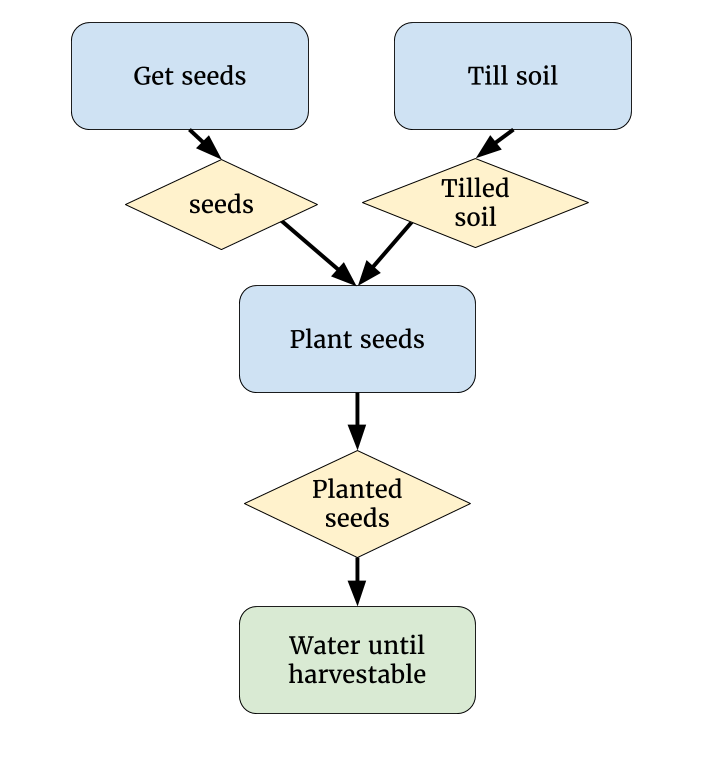
\includegraphics[width=0.4\textwidth]{sdv-grow-crop.png}
%   \quad
%   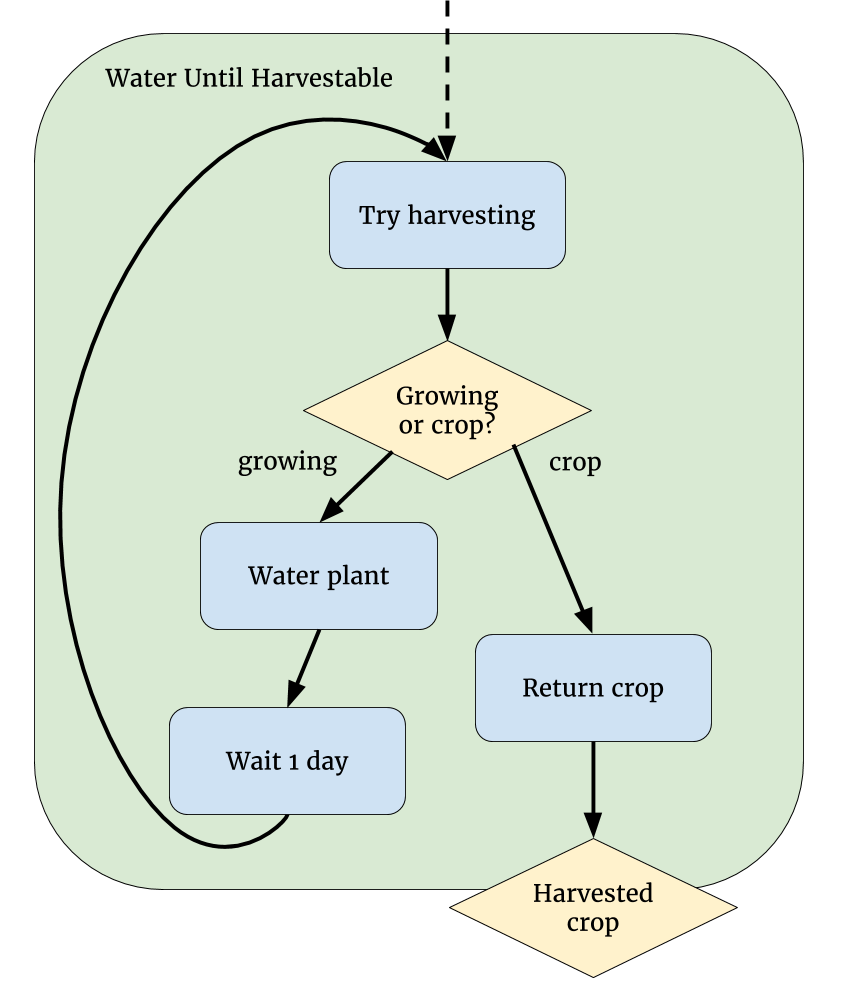
\includegraphics[width=0.4\textwidth]{sdv-water-harvest.png}
%   \caption{Control flow diagrams describing how Stardew Valley skills can
%     be described and composed. Yellow diamond-shaped nodes indicate game
%     responses and resources from the game environment, while blue
%     round-rect nodes are player actions. Green round-rect shapes indicate
%     compound action definitions and invocations.}
% 
% \end{figure*}



% Fishing:
% \begin{verbatim}
% fun get_fish(r:rod, w:water, nf:notfishing) 
% : rod * water * notfishing * fish
% =
%   do  
%     go_fish(r,w,nf)
%   recv <r:rod, w:water, ft : (fish*notfishing)+(trash*notfishing)>.
%     case ft of
%       inl <f, nf> => <r, w, nf, f>
%     | inr <t, nf> => do dispose t recv (). get_fish(r,w,nf)
% \end{verbatim}
% 




\section{Conclusion}
%% Possible things to include:
% - Staged syntax - how to capture? (e.g. "take..." "take what?" "ball"
%   or Prom Week's 2 step interaction formation (select actor, then select
%   who they are acting on))
% - Context-dependent vs. acontextual syntax and its correspondence with
%   the interface stack (hardware inputs vs. linguistic intent - actions
%   performed repeatedly by the player vs. strategies applied to specific
%   pieces of the environment)

Having established a vocabulary of syntax and semantics for player
languages, we can now revisit the potential benefits of this account
mentioned in the introduction and discuss them in more detail.

\subsection{Compositionality for play traces and player skills}

One of the major things that a programming language account provides is
{\em compositionality}: a system for making sense of meaning of a complex
artifact in terms of the meaning of its pieces. This comes up in two places
for looking at games:

{\bf Structured play traces.} With a formalized game language, the sequence
of steps along the transition system described by the operational semantics
forms a mathematical artifact that is subject to deeper analysis than what
can be gained simply from screen or input device recordings. For example,
we can carry out causal analysis, asking ``why'' queries of trace data,
e.g. ``Why was the player able to unlock the door before defeating the boss?'',
as well as filtering traces for desired properties: ``Show me a play trace
where the player used something other than the torch to light the room.''
The recent PlaySpecs project~\cite{osborn2015playspecs} suggests interest
in formulating traces this way to support this kind of query.

{\bf Player skills as programs.} While a play trace may be interpreted as a
straight-line program, even more interesting is the idea of latent
structure in player actions, such as composing multiple low-level game
actions into a higher-level skill, following the cognitive idea of
``chunking.'' We map this idea onto that of {\em functions} in the
programming language that take arguments, generalizing over state space
possibilities (e.g.: the red key opened the red door, so for all colors
$C$, a $C$ key will open a $C$ door). Further reasoning forms like case
analysis to handle unpredictable game behavior and repeating an action
until a condition holds are also naturally expressed as programming
language constructs.


\subsection{Abstraction boundaries between input and mechanics}

% (XXX provide evidence, and or more detail?)

Formalizing game interfaces gives us the tools to explore alternative
interfaces to the same underlying mechanics, without needing to port
game logic between different graphical interface frameworks. For example,
the interactive fiction community has been exploring alternatives to the
two traditional dichotomy of ``parser vs. hypertext'' for presenting
text-based games and interactive story-worlds. An abstraction boundary
between the underlying mechanics, map, and narrative of the world, and the
view and input mechanisms used to interact with it, could open the doors to
research on user interfaces that support players' mental models of a world
conveyed in text.

\subsection{Enabling co-creative play}

Finally, a PL formulation of player actions along with appropriate
composition operators (parallel and sequential composition, branching, and
passing resource dependencies) provides a ``scripting language for free''
to the game environment. 
Such a language can be used to test the game, provided as a game mechanic
as in BOTS, or provided as an optional augmentation to the game's mechanics
for the sake of modding or adding new content to the game world. Especially
in networked game environments, like multi-user domains, massively
multiplayer online games, and social spaces like Second Life, the ability
for the player to program not just her avatar but parts of the game world
itself introduces new opportunities for creative and collaborative play.
Our framework suggests a new approach to designing these affordances for
players in a way that is naturally derived from the game's existing
mechanics and interface.  In the spirit of {\em celebrating the player},
this year's conference theme, we wish to enable the player as a
co-designer of her own game experience.


\subsection{Future Work}
  % Future work: try to draw further analogies. Better REPLs for PLs? 
  In future work, we intend to build software for realizing game language
  designs and experimenting with protocol-based game AI developed as
  programs in these languages. In another direction, we aim to innovate in
  PL design outside of games, such as read-eval-print loops (REPLs) for
  live programming that includes rapid feedback loops motivated by
  gameplay, as well as distributed and concurrent systems that may benefit
  from the protocol-based approach proposed here.


  
% \section{Conclusion}
% 
%   % Summary of contributions (new ideas, why they matter)
% 
% Our primary contribution is an account of {\em input languages} as the
% space between hardware control schemes and a game's mechanics, together
% with a proposal for a rigorous methodology to support designing, analyzing,
% and constructing such languages.
% 

  

% \begin{acks}
%   acknowledgements
% \end{acks}

\bibliographystyle{ACM-Reference-Format}
\bibliography{main,adapton} 

\end{document}

%%% unused
% The language
% a player speaks and the language a game speaks serve somewhat different
% purposes: a game's language includes the visual, textual, and audio
% feedback mechanisms, including semiotic information such as health bars and
% question mark symbols. Such a language is best studied with an
% On the other hand,
% the language the player speaks toward a digital game is formal and
% unambiguous.  understanding of linguistics, psychology, and design. 

% Just as the field of film studies has developed a notion of {\em
% vocabulary} that visual storytellers use to communicate with audiences,
% such as the cinematic device of {\em intercutting} used to convey
% simultaneous action,
% scholars have studied the vocabulary and representational conventions of
% games (XXX cite something re games literacy? salen and zimmerman?) that
% designers employ to communicate with players, such a horizontal green bar
% floating above an avatar representing its health or a question mark
% labeling an object as a reward or power-up. In interactive media, we also
% adopt the notion of {\em affordances} in terms of what kinds of actions
% these representations invite: a health bar above an avatar suggests it may
% be attacked, whereas a question mark labeling a box suggests it might be
% opened.
% % Designers term these representational conventions taken as a
% % systemic whole a {\em design language} (XXX cite?) 
% %
% We have recognized that a symbolic, discretized and representational
% approach to looking at these design decisions has value: the term {\em
% design language} (XXX cite) indicates a recognition that these symbols and
% affordances operate together as a system.
% 
% However, play is a two-way street. Design language explains how the computational half of
% the conversation expresses itself to the human half. This paper introduces
% an account of how the human half of the game loop expresses themselves to
% the computational half.

% (XXX this is kind of a description of the figure)
% play is a two-way street: a game provides affordances for action, a player
% takes action based on those affordances, and the game responds in turn with
% feedback that develops the player's mental model for the behavior of the system
% implied by the interaction as a whole. And, 


